% Fig. 3: Test-fold AUROC on MIMIC-IV for nine models and three tasks (vector, Times 8 pt).
% Values are those reported in the original submission (Fig. 4 and Table III).
\documentclass[10pt,border=1pt]{standalone}
\usepackage{mathptmx}
\usepackage{pgfplots}
\pgfplotsset{compat=1.17}
\begin{document}
\footnotesize
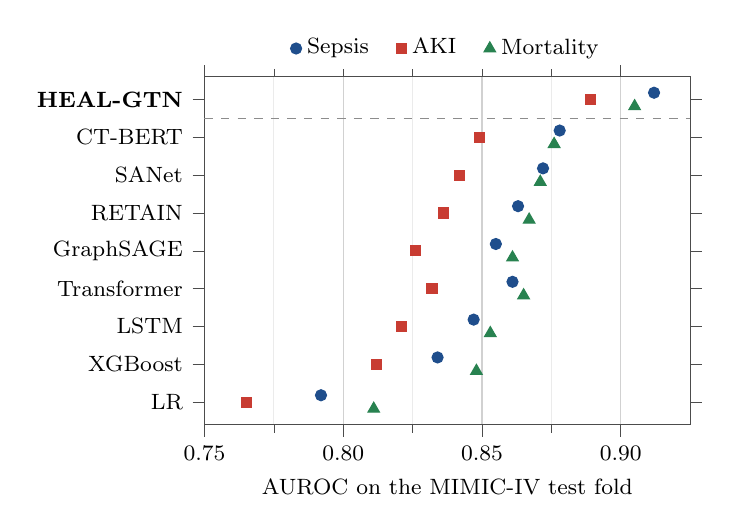
\begin{tikzpicture}
\begin{axis}[
  width=7.75cm, height=6.0cm,
  scale only axis=false,
  xmin=0.75, xmax=0.925,
  ymin=0.4, ymax=9.6,
  xtick={0.75,0.80,0.85,0.90},
  xticklabel style={/pgf/number format/fixed,/pgf/number format/precision=2,/pgf/number format/fixed zerofill},
  minor x tick num=1,
  xmajorgrids, xminorgrids,
  major grid style={draw=black!18, line width=0.4pt},
  minor grid style={draw=black!8, line width=0.3pt},
  ytick={1,...,9},
  yticklabels={LR, XGBoost, LSTM, Transformer, GraphSAGE, RETAIN, SANet, CT-BERT, \textbf{HEAL-GTN}},
  y tick label style={font=\footnotesize},
  tick label style={font=\footnotesize},
  xlabel={AUROC on the MIMIC-IV test fold},
  xlabel style={font=\footnotesize},
  tick align=outside, tick style={black!70},
  axis line style={black!70},
  legend style={font=\footnotesize, at={(0.5,1.02)}, anchor=south, legend columns=3,
                draw=none, /tikz/every even column/.append style={column sep=8pt}},
  legend cell align=left,
  clip=false,
]
\addplot[only marks, mark=*, mark size=2.0pt, color={rgb,255:red,31;green,78;blue,140}]
  coordinates {(0.792,1.18) (0.834,2.18) (0.847,3.18) (0.861,4.18) (0.855,5.18) (0.863,6.18) (0.872,7.18) (0.878,8.18) (0.912,9.18)};
\addlegendentry{Sepsis}
\addplot[only marks, mark=square*, mark size=1.8pt, color={rgb,255:red,200;green,60;blue,50}]
  coordinates {(0.765,1) (0.812,2) (0.821,3) (0.832,4) (0.826,5) (0.836,6) (0.842,7) (0.849,8) (0.889,9)};
\addlegendentry{AKI}
\addplot[only marks, mark=triangle*, mark size=2.4pt, color={rgb,255:red,40;green,130;blue,80}]
  coordinates {(0.811,0.82) (0.848,1.82) (0.853,2.82) (0.865,3.82) (0.861,4.82) (0.867,5.82) (0.871,6.82) (0.876,7.82) (0.905,8.82)};
\addlegendentry{Mortality}
% separator between baselines and the proposed model
\draw[black!45, dashed, line width=0.4pt] (axis cs:0.75,8.5) -- (axis cs:0.925,8.5);
\end{axis}
\end{tikzpicture}
\end{document}
